% !TeX spellcheck = en_US
\chapter{Image Processing}

\section{Linear Filters}
Types of noise:
\begin{itemize}
	\item Salt \& pepper noise
	\item Impulse noise
	\item Gaussian noise\\
	$noise = randn(size(img)) \times \sigma$\\
	$output = img + noise$
	\item \hlr{\underline{Basic assumption:}} \ac{iid}
\end{itemize}
Types of filter:
\begin{itemize}
	\item Correlation Filter: $\displaystyle G[i,j] = \frac{1}{(2k+1)^2} \sum_{u=-k}^{k} \sum_{v=-k}^{k} F[i+u, j+v] $\\
	different weights: $\displaystyle G[i,j] = \sum_{u=-k}^{k} \sum_{v=-k}^{k} H[u,v]F[i+u, j+v] \Rightarrow {\color{red} \boxed{G = H \otimes F}}$\\
	with $H[u,v]$ as non-uniform weights\\
	\hlb{Matlab:} \texttt{filter2, imfilter}
	\item Convolution: \tab $\displaystyle G[i,j] = \sum_{u=-k}^{k} \sum_{v=-k}^{k} H[u,v]F[i-u, j-v] \Rightarrow {\color{red} \boxed{G = H * F}}$\\
	\hlb{Matlab:} \texttt{conv2}\\
	\hlr{If $H[u,v] = H[-u,-v] \Rightarrow$ correlation $\equiv$ convolution}
	\item Averaging Filter: \hlr{Ringing Artifacts??}
	\item Gaussian Filter: $\displaystyle \frac{1}{\sqrt{2\pi}} \exp \left(-\frac{(x-\mu)^2}{2\sigma^2}\right)$\\
	\hlb{Rule of thumb:} set the filter width to $6\sigma$\\
	\hlr{More noise $\Rightarrow\;\; \uparrow \sigma \Rightarrow$ blurring effect}
\end{itemize}

\note
\begin{itemize}
	\item \hlr{$k$ is from the window size $(2k+1)\times(2k+1)$}
	\item \hlr{Efficient implementation:} if filter is separable $\Rightarrow$ apply 1D filter 2 times to have a 2D filter $\Rightarrow$ Reduce the computational cost from $\mathcal{O}(K^2)$ to $\mathcal{O}(2K)$, with $K$ as the kernel size
	\item When coding with \texttt{Python}, the origin of image plane is top left corner, $x$-axis goes left, $y$-axis goes downward (\figref{fig:image-coords})
	\begin{figure}[!htb]
		\centering
		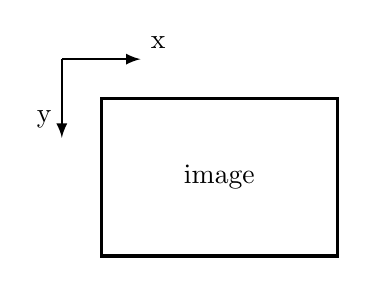
\begin{tikzpicture}			
			\draw[thick,-latex] (0,0) -- (1,0) node[anchor=south west] {x};
			\draw[thick,-latex] (0,0) -- (0,-1) node[anchor=south east] {y};
			\draw[very thick] (0.5,-0.5)  rectangle (3.5,-2.5) node[pos=.5]{image};
		\end{tikzpicture}
		\caption{Image coordinate system in \texttt{Python}}	
		\label{fig:image-coords}
	\end{figure}
	\item Boundary issues:
	\begin{align*}
		&\text{- Full: }  \tab \text{output size} = f+g && 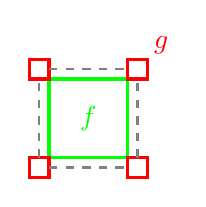
\begin{tikzpicture}[scale=0.5]\draw[green, very thick] (0,0) rectangle (2,2) node[pos=.5]{$f$};
			\draw[red, very thick] (2,2) rectangle (2.5,2.5) node[pos=1.7]{$g$};
			\draw[red, very thick] (0,0) rectangle (-.5,-.5);
			\draw[red, very thick] (2,0) rectangle (2.5,-.5);
			\draw[red, very thick] (0,2) rectangle (-.5,2.5);
			\draw[gray, thick, dashed] (-.25,0) -- (-.25,2);
			\draw[gray, thick, dashed] (0,-.25) -- (2,-.25);
			\draw[gray, thick, dashed] (2.25,0) -- (2.25,2);
			\draw[gray, thick, dashed] (0,2.25) -- (2,2.25);
		\end{tikzpicture}\\
		&\text{- Same:}  \tab \text{output size} = f   && 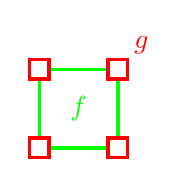
\begin{tikzpicture}[scale=0.5]\draw[green, very thick] (0,0) rectangle (2,2) node[pos=.5]{$f$};
			\draw[red, very thick, fill=white] (1.75,1.75) rectangle (2.25,2.25) node[pos=1.7]{$g$};
			\draw[red, very thick, fill=white] (1.75,-.25) rectangle (2.25,.25);
			\draw[red, very thick, fill=white] (-.25,-.25) rectangle (.25,.25);
			\draw[red, very thick, fill=white] (-.25,1.75) rectangle (.25,2.25);
		\end{tikzpicture}\\
		&\text{- Valid:} \tab \text{output size} = f-g && 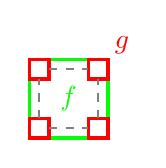
\begin{tikzpicture}[scale=0.5]\draw[green, very thick] (0,0) rectangle (2,2) node[pos=.5]{$f$};
			\draw[red, very thick] (1.5,1.5) rectangle (2,2) node[pos=1.7]{$g$};
			\draw[red, very thick] (0,0) rectangle (.5,.5);
			\draw[red, very thick] (2,0) rectangle (1.5,.5);
			\draw[red, very thick] (0,2) rectangle (.5,1.5);
			\draw[gray, thick, dashed] (.5,.25) -- (1.5,0.25);
			\draw[gray, thick, dashed] (.25,.5) -- (.25,1.5);
			\draw[gray, thick, dashed] (1.75,.5) -- (1.75,1.5);
			\draw[gray, thick, dashed] (.5,1.75) -- (1.5,1.75);
		\end{tikzpicture}
	\end{align*}
	\hlb{Pixel near boundary}:
	\begin{itemize}
		\item Clip filter (black) $\Rightarrow$ dark border
		\item Wrap around
		\item Copy edge $\Rightarrow$ Strong edge response
		\item Reflect across edge
	\end{itemize}
	\item Correlation \ac{vs} convolution:
	\begin{itemize}
		\item Both are linear shift invariant \ac{LSI}:\\
		\tab $h \circ (f_0 + f_1) = h \circ f_1 + h \circ f_0$
		\item Conv is better, it has additional nice properties
		\begin{itemize}
			\item commutative: $f*g = g*f$
			\item associative: $(f*g)*h = f*(g*h)$
			\item Fourier transform $f*g \multimap F.G$ and $f.h \multimap F*H$
		\end{itemize}
		\item With impulse image, Conv reproduces itself, while Corr reflects itself.
	\end{itemize}	
\end{itemize}

\section{Background}
\label{sec:filter-background}
\begin{itemize}
	\item Taking the Fourier Transform of a signal $\Rightarrow$ Frequency coefficients $\Rightarrow$ \hlb{Frequency Spectrum}\\
	\hlr{\underline{Duality:}} $\;$The \hlr{better} a function is \hlr{localized} in one domain\\
	\tab\tab the \hlr{worse} it is \hlr{localized} in the other domain.
	\item Effect of Convolution: $ f * g \multimap F \cdot G$\\
	taking convolution in one domain is equivalent to multiplication in the other domain\\
	A Guassian has compact support in both domains\\
	$\Rightarrow$ \hlb{convenient choice} for \hlr{low-pass filter}
	\item Sharpening filter \hlr{(high-pass filter)}: emphasizes noise as well, since noise is high \ac{freq} signal.
\end{itemize}
\begin{figure}[!htb]
	\centering
	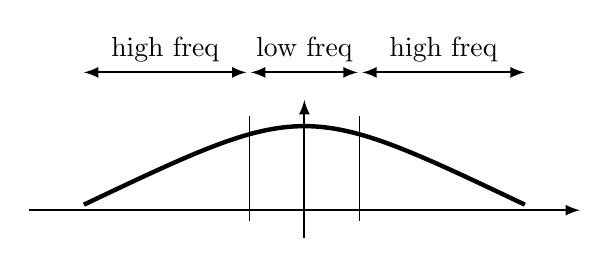
\begin{tikzpicture}[scale=0.7]
		\draw[thick,-latex] (-5,0) -- (5,0);
		\draw[thick,-latex] (0,-.5) -- (0,2);
		\draw[ultra thick] (-4,.1) .. controls (0,2) .. (4,.1);
		\draw[thin] (-1,-.2) -- (-1,1.7);
		\draw[thin] (1,-.2)  -- (1,1.7);
		\draw[thick,latex-latex] (-4,2.5) -- (-1.05,2.5) node[pos=0.5, above=0.2]{high \ac{freq}};
		\draw[thick,latex-latex] (1.05,2.5) -- (4,2.5) node[pos=0.5, above=0.2]{high \ac{freq}};
		\draw[thick,latex-latex] (-0.97,2.5) -- (0.97,2.5) node[pos=0.5, above=0.2]{low \ac{freq}};
	\end{tikzpicture}
	\caption{Frequency domain (Fourier).}
	\label{fig:freq-domain}
\end{figure}

\section{Non-Linear Filters}
\begin{itemize}
	\item Median filter: replace each pixel by the median of the neighbors.
	\begin{itemize}
		\item \hlr{remove spikes} (good for impulse, salt \& pepper noise)
		\item \hlr{edge preserving} (unlike mean filter)
	\end{itemize}
	\note If we increase the Median filter's filter size $\Rightarrow$ reduce structure and loose details
\end{itemize}

\section{Multi-Scale Representations}
\begin{itemize}
	\item Image pyramid: very \hlb{little overhead} (in terms of \hlb{computational cost}).
	\item \hlb{Fourier Interpretation:} Discrete Sampling\\
	Sampling in spatial domain is like \hlb{multiplying with a spike \ac{func}}.
	
	\begin{figure}[!htb]
		\centering
		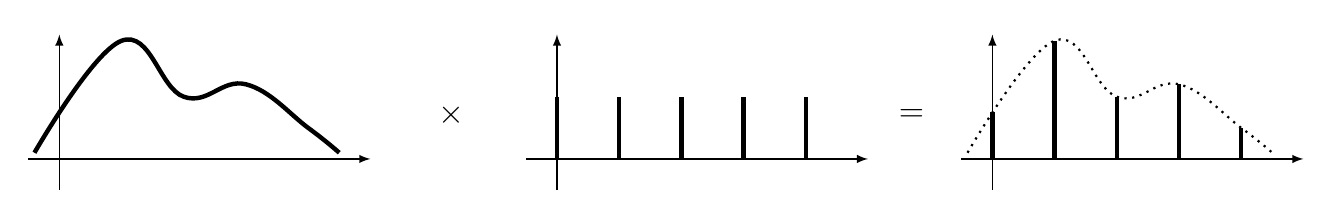
\begin{tikzpicture}[scale=0.79]
			\draw[-latex] (-.5,0) -- (5,0);
			\draw[-latex] (0,-.5) -- (0,2);
			\draw[ultra thick] plot [smooth, tension=.7] coordinates {(-.4,.1) (1,1.9) (2,1) (3,1.2) (4, .5) (4.5,0.1)};
			\node at (6.3,.7) {\large{$\boldsymbol{\times}$}};
			\draw[-latex] (7.5,0) -- (13,0);
			\draw[-latex] (8,-.5) -- (8,2);
			\draw[ultra thick] (8 ,0) -- (8 ,1);
			\draw[ultra thick] (9 ,0) -- (9 ,1);
			\draw[ultra thick] (10,0) -- (10,1);
			\draw[ultra thick] (11,0) -- (11,1);
			\draw[ultra thick] (12,0) -- (12,1);		
			\node at (13.7,.7) {\large{$\boldsymbol{=}$}};
			
			\draw[-latex] (14.5,0) -- (20,0);
			\draw[-latex] (15,-.5) -- (15,2);
			\draw[dotted, thick] plot [smooth, tension=.7, dashed] coordinates {(14.6,.1) (16,1.9) (17,1) (18,1.2) (19, .5) (19.5,.1)};
			\draw[ultra thick] (15,0) -- (15,.75);
			\draw[ultra thick] (16,0) -- (16,1.9);
			\draw[ultra thick] (17,0) -- (17,1);
			\draw[ultra thick] (18,0) -- (18,1.2);
			\draw[ultra thick] (19,0) -- (19,.5);
		\end{tikzpicture}
	\end{figure}
	
	$\Rightarrow$ Sampling in the frequency domain is like \hlb{convolving with a spike \ac{func}}.
	\begin{figure}[!htb]
		\centering
		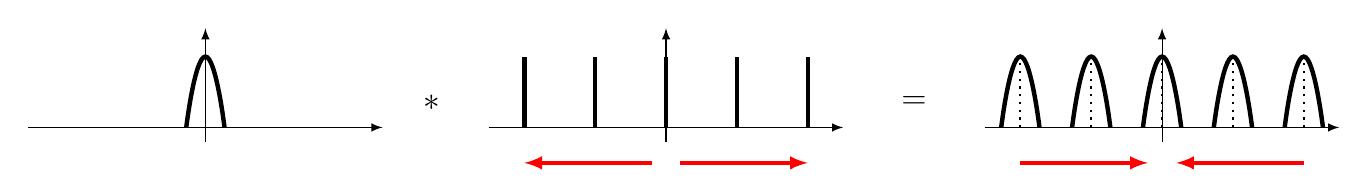
\begin{tikzpicture}[scale=0.9]
			\draw[-latex] (-2.5,0) -- (2.5,0);
			\draw[-latex] (0,-.2) -- (0,1.4);
			\draw[ultra thick] plot [smooth, tension=1] coordinates {(-.27,0) (0,1) (.27,0)};		
			\node at (3.2,.35) {\large{$\boldsymbol{\ast}$}};
			\draw[-latex] (4,0) -- (9,0);
			\draw[-latex] (6.5,-.2) -- (6.5,1.4);
			\draw[ultra thick] (4.5,0) -- (4.5,1);
			\draw[ultra thick] (5.5,0) -- (5.5,1);
			\draw[ultra thick] (6.5,0) -- (6.5,1);
			\draw[ultra thick] (7.5,0) -- (7.5,1);
			\draw[ultra thick] (8.5,0) -- (8.5,1);
			\node at (10 ,.35) {\large{$\boldsymbol{=}$}};		
			\draw[-latex] (11,0) -- (16,0);
			\draw[-latex] (13.5,-.2) -- (13.5,1.4);
			\draw[dotted, thick] (11.5,0) -- (11.5,1);
			\draw[dotted, thick] (12.5,0) -- (12.5,1);
			\draw[dotted, thick] (13.5,0) -- (13.5,1);
			\draw[dotted, thick] (14.5,0) -- (14.5,1);
			\draw[dotted, thick] (15.5,0) -- (15.5,1);
			\draw[ultra thick] plot [smooth, tension=1] coordinates {(11.23,0) (11.5,1) (11.77,0)};
			\draw[ultra thick] plot [smooth, tension=1] coordinates {(12.23,0) (12.5,1) (12.77,0)};
			\draw[ultra thick] plot [smooth, tension=1] coordinates {(13.23,0) (13.5,1) (13.77,0)};
			\draw[ultra thick] plot [smooth, tension=1] coordinates {(14.23,0) (14.5,1) (14.77,0)};
			\draw[ultra thick] plot [smooth, tension=1] coordinates {(15.23,0) (15.5,1) (15.77,0)};
			\draw[red, latex-, very thick] (4.5,-.5) -- (6.3,-.5);
			\draw[red, -latex, very thick] (6.7,-.5) -- (8.5,-.5);
			\draw[red, -latex, very thick] (11.5,-.5) -- (13.3,-.5);
			\draw[red, latex-, very thick] (13.7,-.5) -- (15.5,-.5);		
		\end{tikzpicture}
	\end{figure}\\
	$\Rightarrow$ when we sampling with lower \ac{freq}, the spikes will get further from each others. Due to duality in \secref{sec:filter-background}, the magnitude spectrum will be overlapped $\Rightarrow$ we will not be able to reconstruct the original signal / data.
	\item \hlb{Nyquist theorem and limit:} to recover a certain \ac{freq} $f$, you have to take sample with at least with $2f$.\\	
	\hlr{$\Rightarrow$ Aliasing artifacts in Graphics:} overlapped signal (because sampling with too low frequency)\\	
	\note We can't recover high \ac{freq} (edges), but we can \hlb{avoid artifacts} by \hlb{prior smoothing} before sampling.
	\item The Gaussian Pyramid:	perform blurring \& smoothing $\Rightarrow$ then down-sampling \todo{Image}
	\item The Laplacian Pyramid: \todo{Image}
	\begin{align*}
		L_i &= G_i - expand(G_{i+1})\\
		G_i &= L_i + expand(G_{i+1})\\
		L_n &= G_n
	\end{align*}
	$\Rightarrow L_{0} \rightarrow L_{n-1}$ contain \hlb{high \ac{freq} \ac{info}}\\
	\note Images in Laplacian Pyramid \hlb{can be compressed further} than the corresponding Gaussian Pyramid images.
	\item \hlr{Laplacian $\sim$ Difference of Gaussians}\\
	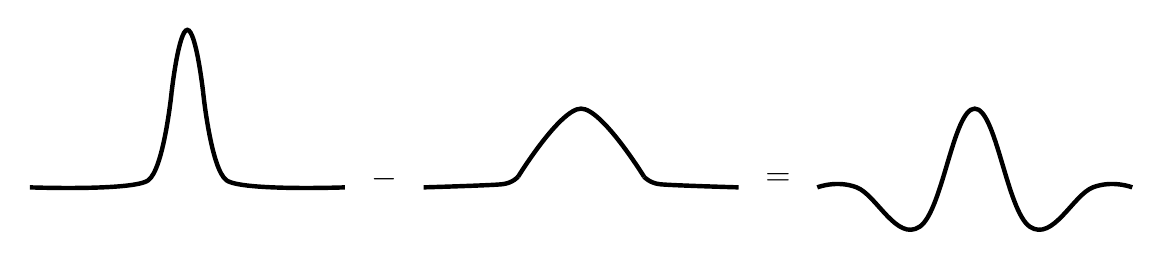
\begin{tikzpicture}
		\draw[ultra thick] plot [smooth, tension=1] coordinates {(-.2,1.21) (0,2) (.2,1.21)};
		\draw[ultra thick] plot [smooth, tension=.4] coordinates {(-2,0) (-.5,.0876) (-.2,1.21)};
		\draw[ultra thick] plot [smooth, tension=.4] coordinates {(.2,1.21) (.5,.0876) (2,0)};
		\node at (2.5,.1) {\large{$\boldsymbol{-}$}};
		\draw[ultra thick] plot [smooth, tension=.6] coordinates {(-.8+5,.135) (0+5,1) 	  (.8+5,.135)};		
		\draw[ultra thick] plot [smooth, tension=.4] coordinates {(-2 +5,0)   (-1+5,.04) (-.8+5,.135)};
		\draw[ultra thick] plot [smooth, tension=.4] coordinates {(.8 +5,.135) (1+5,.04)   (2+5,0)};
		\node at (7.5,.1) {\large{$\boldsymbol{=}$}};
		\draw[ultra thick] plot [smooth, tension=.7] coordinates {(-2+10,0) (-1.5+10,0) (-.7+10,-.5) (0+10,1) (.7+10,-.5) (1.5+10,0) (2+10,0)};
	\end{tikzpicture}\\
	$\Rightarrow$ detect high-\ac{freq} $\approx$ edges\\
	The name Laplace $\Rightarrow$ from a combinations of 2nd derivatives\\
	Laplacian: $\displaystyle {\color{red} \boxed{\nabla^2f = \frac{\partial^2f}{\partial x^2} + \frac{\partial^2f}{\partial y^2}}}$
	\begin{align*}
		\frac{\partial^2f}{\partial x^2} &= [f(x+1,y) - f(x,y)] - [f(x,y) - f(x-1,y)] \\
		&= f(x+1,y) + f(x-1,y) - 2f(x,y) \\
		\Rightarrow \nabla^2f &= f(x\pm1, y) + f(x, y\pm1) - 4f(x,y) \\
	\end{align*}
	$\Rightarrow$ \hlb{Laplacian filter:} \tab 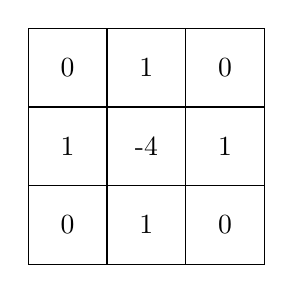
\begin{tikzpicture}
		\draw (0,0) rectangle (1,1) node[pos=.5]{0};
		\draw (1,1) rectangle (2,2) node[pos=.5]{-4};
		\draw (2,2) rectangle (3,3) node[pos=.5]{0};
		\draw (1,0) rectangle (2,1) node[pos=.5]{1};
		\draw (2,0) rectangle (3,1) node[pos=.5]{0};
		\draw (0,1) rectangle (1,2) node[pos=.5]{1};
		\draw (0,2) rectangle (1,3) node[pos=.5]{0};
		\draw (1,2) rectangle (2,3) node[pos=.5]{1};
		\draw (2,1) rectangle (3,2) node[pos=.5]{1};
	\end{tikzpicture}	 
\end{itemize}

\section{Filters as Templates}
Correlation filtering as Template Matching.

\section{Image Gradients}
\begin{itemize}
	\item Differentiation \& Convolution: $\displaystyle \frac{\partial f(x,y)}{\partial x} \approx \frac{f(x+1,y) - f(x,y)}{1}$\\
	$\Rightarrow$ Filter: $\begin{bmatrix}
		1 & -1
	\end{bmatrix}$\\
	\hlb{Problem:} it shifts the image \\
	$\Rightarrow$ Prewitt, Sobel, Robert filters:
	\begin{itemize}
		\item Prewitt filter: $\begin{bmatrix}
			-1 & 0 & 1\\
			-1 & 0 & 1\\
			-1 & 0 & 1
		\end{bmatrix}; \begin{bmatrix}
			1 & 1 & 1\\
			0 & 0 & 0\\
			-1 & -1 & -1
		\end{bmatrix}$
		\item Sobel filter: $M_x=\begin{bmatrix}
			-1 & 0 & 1\\
			-2 & 0 & 2\\
			-1 & 0 & 1
		\end{bmatrix}; M_y=\begin{bmatrix}
			1 & 2 & 1\\
			0 & 0 & 0\\
			-1 & -2 & -1
		\end{bmatrix}$
		\item Robert $\begin{bmatrix}
			0 & 1\\
			-1 & 0
		\end{bmatrix}; \begin{bmatrix}
		1 & 0\\
		0 & -1
	\end{bmatrix}$
	\end{itemize}
	\item With noise, we need to smooth the image first
\end{itemize}

\section{Edge Detection}


\section{Structure Extraction}

\todo{missing content}